\chapter{Multiple Integrals}


In this chapter, we extend this powerful idea into higher dimensions using the tools of multiple integration. While single integration enables us to calculate the area under a curve or the volume under a surface, multiple integration allows us to calculate volumes in three dimensions, and even hypervolumes in higher dimensions.

We start by discussing double integration, which allows us to find the volume under a surface in three dimensions. This method involves slicing the solid into infinitesimally thin disks, and summing the volumes of these disks.

Next, we'll cover triple integration, a tool that lets us find the volume of more complicated solids in three-dimensional space. The idea is similar to double integration, but instead of slicing the solid into disks, we slice it into infinitesimally small cubes.

To properly implement these techniques, we'll also discuss the different coordinate systems that can be used in multiple integration, such as rectangular, cylindrical, and spherical coordinates, and when it's advantageous to use one system over another.

By the end of this chapter, you will have a deeper understanding of the techniques of multiple integration and how to apply them to find the volumes of various types of solids. The methods we study here will serve as a foundation for many topics in higher mathematics and physics, including electromagnetism, fluid dynamics, and quantum mechanics.

\begin{Exercise}[title={Using Polar Coordinates in Multiple Integration}, label=polarmulti]

\Question Use double integration to find the volume of the solid that lies under the surface $z = 4 - x^2 - y^2$ and above the $xy$-plane.

\end{Exercise}
\begin{Answer}[ref=polarmulti]

We are finding the volume of the solid that lies under the surface $z = 4 - x^2 - y^2$ and above the $xy$-plane.

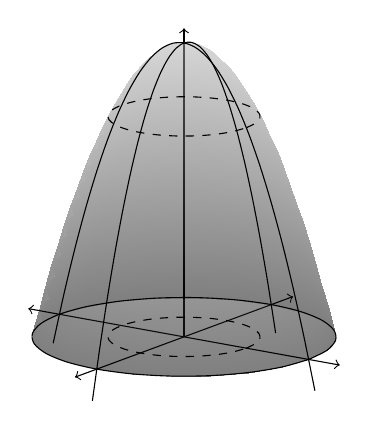
\begin{tikzpicture}
  \begin{axis}[
    view={35}{15},
    unit vector ratio=1 1 1,
    ticks = none,
    axis lines=middle,
    ymin=-2.5,
    ymax=2.5,
    xmax=2.5,
    xmin=-2.5,
    zmin=0,
    zmax=4.2,
    x axis line style=<->,
    y axis line style=<->,
    z axis line style=->,
    clip=false
  ]
    \addplot3[surf,shader=interp,domain=0:360,y domain=0:2, opacity=0.5,
    colormap={blackwhite}{color=(black) color=(black!30)}] ({y*cos(x)},
    {y*sin(x)},{4-y^2});
    \addplot3[samples y=0,domain=0:360,smooth]({2*cos(x)},  {2*sin(x)},0);
    \addplot3[samples y=0,domain=0:360,smooth,dashed]({cos(x)},  {sin(x)},0);
    \addplot3[samples y=0,domain=0:360,smooth,dashed]({cos(x)},  {sin(x)},3);
    \addplot3[samples y=0,domain=-2.1:2.1,smooth](0,  {x},{4 - x^2});
    \addplot3[samples y=0,domain=-2.1:2.1,smooth]({x},0, {4 - x^2});
  \end{axis}
\end{tikzpicture}

We can use polar coordinates to simplify the double integral. In polar coordinates, $x = r\cos(\theta)$ and $y = r\sin(\theta)$, so $x^2 + y^2 = r^2$. The volume under the surface and above the $xy$-plane is given by

\begin{equation}
V = \int \int (4 - r^2) r \, dr \, d\theta,
\end{equation}

where $r$ ranges from 0 to 2 (since $4 - r^2 \geq 0$ if $0 \leq r \leq 2$) and $\theta$ ranges from 0 to $2\pi$.

Hence,

\begin{align*}
V & = \int_{0}^{2\pi} \int_{0}^{2} (4r - r^3) \, dr \, d\theta \\
& = \int_{0}^{2\pi} \left[ 2r^2 - \frac{1}{4}r^4 \right]_{0}^{2} \, d\theta \\
& = \int_{0}^{2\pi} (8 - 4) \, d\theta \\
& = \int_{0}^{2\pi} 4 \, d\theta \\
& = \left[ 4\theta \right]_{0}^{2\pi} \\
& = 8\pi.
\end{align*}

So the volume of the solid is $8\pi$ cubic units.

\end{Answer}


